\chapter{MARTA e il suo modello di mobilita'}

\section{MARTA}

MARTA (MARine Tool for Architecture) e' un veicolo autonomo sottomarino (Autonomous Underwater Vehicle, AUV) sviluppato dall'Universita' di Firenze nell'ambito dell'iniziativa ARROWS, progetto supportato dalla Commissione Europea che aveva come obbiettivo lo sviluppo di tecnologie a basso costo da mettere a disposizione degli archeologi impegnati in ricerche in ambienti sottomarini. \newline
In quest'ottica, MARTA viene pensato come AUV con impiegabile in ruoli di ricerca di punti d'interesse all'interno dell'area archeologica e della loro successiva ispezione (acquisizione di immagini del punto individuato). \newline
Questo risultato viene raggiunto grazie alla natura modulare del progetto di questo AUV, che garantisce un'elevata personalizzabilita' della configurazione operativa del veicolo ( a livello di payload di sensori ottici/acustici, tipo di propulsione, power source). \newline
Inoltre, MARTA viene equipaggiato con due modem acustici, diversi per velocita' di trasmissione/consumo energetico, il che lo rendono adatto a svolgere il ruolo di "ponte" comunicativo per i dispositivi BR (Biometric Robots), solitamenti impegnati ad analizzare le zone piu' difficilmente accessibili dell'area archeologica subacquea.

\begin{figure}[H]
	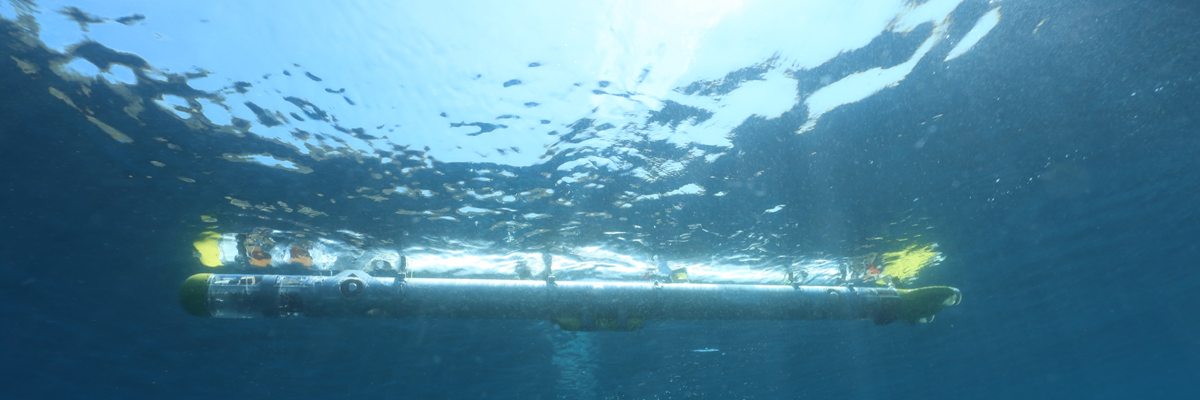
\includegraphics[width=\linewidth]{MARTA.png}
	\caption{MARTA in superficie}
	\label{fig:MARTA}
	\centering
\end{figure}

Per quanto riguarda le dimensioni del veicolo, MARTA ha una lunghezza massima di 3.7m (nella sua configurazione completa), pesa 80 kg fuori dall'acqua ed  ha un diametro esterno di 180mm. \newline
Il movimento del veicolo e' vincolato a 5 gradi di liberta'. \newline Infatti MARTA puo' muoversi in verticale, salendo o scendendo di profondita', ruotare mantenendosi parallelo al piano orizzontale e spostarsi in avanti nella direzione stessa del veicolo, oltre a poter stazionare fisso in punto. La mobilita' del veicolo e' controllata da 6 attuatori, di cui 2 eliche posteriori, due eliche laterali e due eliche verticali. \newline Il veicolo puo' raggiungere una profondita' massima di 120m, viaggiando tipicamente ad una velocita' media di 1 nodo al secondo ( la velocita' massima dichiarata e' di 3 nodi al secondo). \newline 
A livello software, la gestione del veicolo e' affidata al software ROS (Robot Operating System), che presenta un architettura altamente modulare che ben si adatta alla modularita' del design progettuale di MARTA.

\subsection{Implementazione modello di mobilita' di MARTA su SUNSET}
Lo specifico modello di mobilita' di MARTA ha richiesto la necessita' di intervenire sulla gestione della simulazione del movimento di un AUV all'interno del framework di simulazione SUNSET. \newline In particolare, MARTA presenta due vincoli di movimento cui prestare attenzione. In primis, il veicolo in questione non puo' contemporaneamente muoversi in avanti e variare la sua quota di profondita', essendo le due modalita' di spostamento mutuamente esclusive. \newline In secondo luogo, MARTA puo' variare la propria direzione di spostamento sul piano orizzontale solamente in posizione stazionaria, ergo qualunque cambio di direzione richiede preventivamente che il veicolo si fermi e solo in seguito effettui la rotazione necessaria, utilizzando le eliche laterali. \newline
Dati quindi dei generici waypoints, corrispondenti ad un percorso cui si intende vincolare il movimento dell'AUV, si e' voluto, all'interno di SUNSET, far si che il simulatore generasse un nuovo insieme di waypoints, includente l'insieme originario e rappresentante un nuovo percorso che rispettase  i vincoli di movimento introdotti da MARTA. \newline Per far ottenere questo risultato, e' stata creata una specifica funzione in linguaggio Tcl. \newline All'interno di questa vengono iterativamente prese in esame i waypoints passati in input allo script simulativo (salvati all'interno di un apposita variabile globale). \newline Per ciascuna posizione, viene considerata la posizione precedente da cui l'AUV proviene.\newline Se quest'ultima si trova ad una profondita' differente dalla posizione in esame, la funzione aggiunge al percorso dell'AUV un waypoint intermedio, avente come coordinate geografiche proprio quelle del waypoint precedente a quello analizzato ma sito alla stessa profondita' del nodo in esame, dimodoche' il movimento del veicolo avvenga prima lungo la verticale e poi in orizzontale, in maniera consona al modello di movimento di MARTA.\newline
Nella figura sottostante, si consideri il punto B come il waypoint in esame in una specifica iterazione, il punto C la posizione successiva da raggiungere ed il punto A la posizione precedentemente attraversata.\newline $\varphi$  risulta quindi essere l'angolo di cui e' necessario ruotare l'AUV prima di dirigersi verso il nodo C (indipendentemente dal fatto che il nodo C si trovi ad una quota differente rispetto a B). 

\begin{figure}[H]
    \centering
	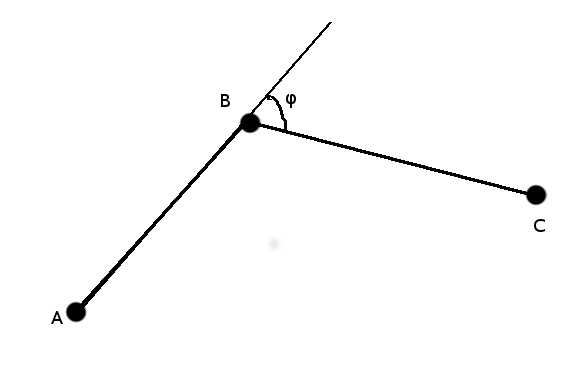
\includegraphics[scale=0.5]{scalarprod.png}
\end{figure}

Per calcolare quest'angolo, si ricorre semplicemente alla formula del prodotto scalare fra due vettori, in questo caso i vettori AB e BC, ottenuti dalle coordinate geografiche dei rispettivi waypoints (previa trasformazione in coordinate cartesiane nel sistema ECEF, Earth Centered Earth Fixed ).\newline Per la formula del prodotto scalare:


\begin{equation}
\overrightarrow{AB} \cdot \overrightarrow{BC} = |AB| |BC| cos{phy}    
\end{equation}

 
Si ottiene cosi' il valore dell'angolo $\varphi$ che, diviso per la velocita' di rotazione dell'AUV, da' la misura del tempo di rotazione impiegato da MARTA per effettuare il cambio di direzione. \newline L'intervallo temporale cosi' calcolato viene passato in input alla funzione di aggiunta del waypoint corrispondente alla posizione B.
\newline Difatti il sistema di gestione dei waypoints, facente parte del framework WOSS, consente di specificare, contestualmente alla creazione di un waypoint, un tempo nel quale l'AUV e' costretto a sostare fermo nella posizione del waypoint.\newline In questo modo, il tempo di rotazione richiesto da MARTA viene trasformato in questo tempo d'attesa, ottenendo come risultato finale un modello di movimento del tutto rispondente ai vincoli imposti dal veicolo in considerato.\newline
Queste trasformazioni sono state applicate ad un percorso "a serpentina", tipico per missioni di perlustrazione/monitoraggio di una certa area marina dai confini ben definiti.\newline
Riportiamo in basso i grafici del percorso dell'AUV non modificato e quello ottenuto imponendo i vincoli di movimento di MARTA.

\begin{figure}[h!]
	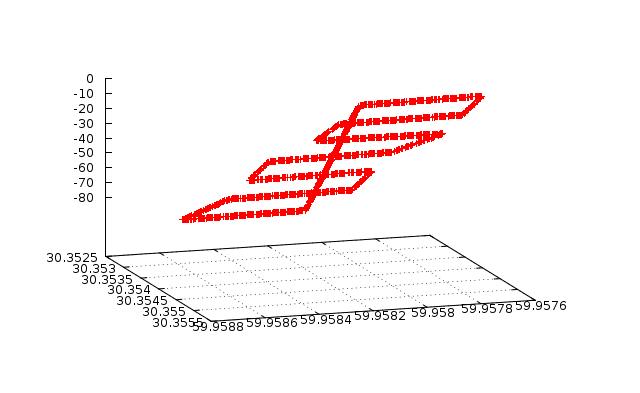
\includegraphics[width=\linewidth]{posizioninoscript.png}
	\caption{Percorso dell'AUV senza vincoli}
	\label{fig:}
	\centering
\end{figure}

\begin{figure}[h!]
	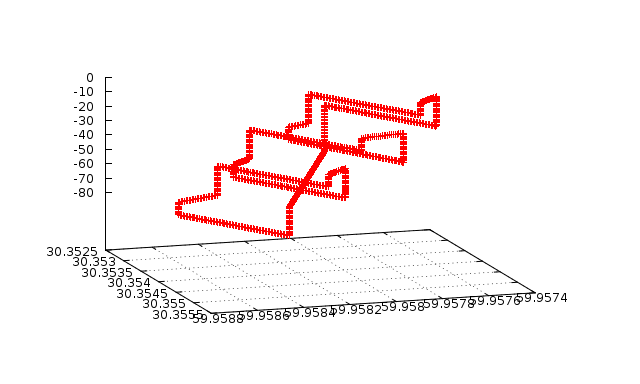
\includegraphics[width=\linewidth]{posizioniscript.png}
	\caption{Percorso dell'AUV con vincoli}
	\label{fig:}
	\centering
\end{figure}